\documentclass[]{book}
\usepackage{lmodern}
\usepackage{amssymb,amsmath}
\usepackage{ifxetex,ifluatex}
\usepackage{fixltx2e} % provides \textsubscript
\ifnum 0\ifxetex 1\fi\ifluatex 1\fi=0 % if pdftex
  \usepackage[T1]{fontenc}
  \usepackage[utf8]{inputenc}
\else % if luatex or xelatex
  \ifxetex
    \usepackage{mathspec}
  \else
    \usepackage{fontspec}
  \fi
  \defaultfontfeatures{Ligatures=TeX,Scale=MatchLowercase}
\fi
% use upquote if available, for straight quotes in verbatim environments
\IfFileExists{upquote.sty}{\usepackage{upquote}}{}
% use microtype if available
\IfFileExists{microtype.sty}{%
\usepackage{microtype}
\UseMicrotypeSet[protrusion]{basicmath} % disable protrusion for tt fonts
}{}
\usepackage[unicode=true]{hyperref}
\PassOptionsToPackage{usenames,dvipsnames}{color} % color is loaded by hyperref
\hypersetup{
            pdftitle={Saemix: Open Source R package for mixed effects modeling},
            pdfauthor={Marc Lavielle, Emmanuelle Comets, Audrey Lavenu and Belhal Karimi},
            colorlinks=true,
            linkcolor=Maroon,
            citecolor=Blue,
            urlcolor=blue,
            breaklinks=true}
\urlstyle{same}  % don't use monospace font for urls
\usepackage{natbib}
\bibliographystyle{apalike}
\usepackage{color}
\usepackage{fancyvrb}
\newcommand{\VerbBar}{|}
\newcommand{\VERB}{\Verb[commandchars=\\\{\}]}
\DefineVerbatimEnvironment{Highlighting}{Verbatim}{commandchars=\\\{\}}
% Add ',fontsize=\small' for more characters per line
\usepackage{framed}
\definecolor{shadecolor}{RGB}{248,248,248}
\newenvironment{Shaded}{\begin{snugshade}}{\end{snugshade}}
\newcommand{\KeywordTok}[1]{\textcolor[rgb]{0.13,0.29,0.53}{\textbf{{#1}}}}
\newcommand{\DataTypeTok}[1]{\textcolor[rgb]{0.13,0.29,0.53}{{#1}}}
\newcommand{\DecValTok}[1]{\textcolor[rgb]{0.00,0.00,0.81}{{#1}}}
\newcommand{\BaseNTok}[1]{\textcolor[rgb]{0.00,0.00,0.81}{{#1}}}
\newcommand{\FloatTok}[1]{\textcolor[rgb]{0.00,0.00,0.81}{{#1}}}
\newcommand{\ConstantTok}[1]{\textcolor[rgb]{0.00,0.00,0.00}{{#1}}}
\newcommand{\CharTok}[1]{\textcolor[rgb]{0.31,0.60,0.02}{{#1}}}
\newcommand{\SpecialCharTok}[1]{\textcolor[rgb]{0.00,0.00,0.00}{{#1}}}
\newcommand{\StringTok}[1]{\textcolor[rgb]{0.31,0.60,0.02}{{#1}}}
\newcommand{\VerbatimStringTok}[1]{\textcolor[rgb]{0.31,0.60,0.02}{{#1}}}
\newcommand{\SpecialStringTok}[1]{\textcolor[rgb]{0.31,0.60,0.02}{{#1}}}
\newcommand{\ImportTok}[1]{{#1}}
\newcommand{\CommentTok}[1]{\textcolor[rgb]{0.56,0.35,0.01}{\textit{{#1}}}}
\newcommand{\DocumentationTok}[1]{\textcolor[rgb]{0.56,0.35,0.01}{\textbf{\textit{{#1}}}}}
\newcommand{\AnnotationTok}[1]{\textcolor[rgb]{0.56,0.35,0.01}{\textbf{\textit{{#1}}}}}
\newcommand{\CommentVarTok}[1]{\textcolor[rgb]{0.56,0.35,0.01}{\textbf{\textit{{#1}}}}}
\newcommand{\OtherTok}[1]{\textcolor[rgb]{0.56,0.35,0.01}{{#1}}}
\newcommand{\FunctionTok}[1]{\textcolor[rgb]{0.00,0.00,0.00}{{#1}}}
\newcommand{\VariableTok}[1]{\textcolor[rgb]{0.00,0.00,0.00}{{#1}}}
\newcommand{\ControlFlowTok}[1]{\textcolor[rgb]{0.13,0.29,0.53}{\textbf{{#1}}}}
\newcommand{\OperatorTok}[1]{\textcolor[rgb]{0.81,0.36,0.00}{\textbf{{#1}}}}
\newcommand{\BuiltInTok}[1]{{#1}}
\newcommand{\ExtensionTok}[1]{{#1}}
\newcommand{\PreprocessorTok}[1]{\textcolor[rgb]{0.56,0.35,0.01}{\textit{{#1}}}}
\newcommand{\AttributeTok}[1]{\textcolor[rgb]{0.77,0.63,0.00}{{#1}}}
\newcommand{\RegionMarkerTok}[1]{{#1}}
\newcommand{\InformationTok}[1]{\textcolor[rgb]{0.56,0.35,0.01}{\textbf{\textit{{#1}}}}}
\newcommand{\WarningTok}[1]{\textcolor[rgb]{0.56,0.35,0.01}{\textbf{\textit{{#1}}}}}
\newcommand{\AlertTok}[1]{\textcolor[rgb]{0.94,0.16,0.16}{{#1}}}
\newcommand{\ErrorTok}[1]{\textcolor[rgb]{0.64,0.00,0.00}{\textbf{{#1}}}}
\newcommand{\NormalTok}[1]{{#1}}
\usepackage{longtable,booktabs}
\usepackage{graphicx,grffile}
\makeatletter
\def\maxwidth{\ifdim\Gin@nat@width>\linewidth\linewidth\else\Gin@nat@width\fi}
\def\maxheight{\ifdim\Gin@nat@height>\textheight\textheight\else\Gin@nat@height\fi}
\makeatother
% Scale images if necessary, so that they will not overflow the page
% margins by default, and it is still possible to overwrite the defaults
% using explicit options in \includegraphics[width, height, ...]{}
\setkeys{Gin}{width=\maxwidth,height=\maxheight,keepaspectratio}
\IfFileExists{parskip.sty}{%
\usepackage{parskip}
}{% else
\setlength{\parindent}{0pt}
\setlength{\parskip}{6pt plus 2pt minus 1pt}
}
\setlength{\emergencystretch}{3em}  % prevent overfull lines
\providecommand{\tightlist}{%
  \setlength{\itemsep}{0pt}\setlength{\parskip}{0pt}}
\setcounter{secnumdepth}{5}
% Redefines (sub)paragraphs to behave more like sections
\ifx\paragraph\undefined\else
\let\oldparagraph\paragraph
\renewcommand{\paragraph}[1]{\oldparagraph{#1}\mbox{}}
\fi
\ifx\subparagraph\undefined\else
\let\oldsubparagraph\subparagraph
\renewcommand{\subparagraph}[1]{\oldsubparagraph{#1}\mbox{}}
\fi
\usepackage{booktabs}
\usepackage{amsthm}
\makeatletter
\def\thm@space@setup{%
  \thm@preskip=8pt plus 2pt minus 4pt
  \thm@postskip=\thm@preskip
}
\makeatother

\title{\texttt{Saemix}: Open Source R package for mixed effects modeling}
\author{Marc Lavielle, Emmanuelle Comets, Audrey Lavenu and Belhal Karimi}
\date{2020-01-28}

\begin{document}
\maketitle

{
\hypersetup{linkcolor=black}
\setcounter{tocdepth}{1}
\tableofcontents
}
\chapter*{Saemix: R package for mixed effects
modeling}\label{saemix-r-package-for-mixed-effects-modeling}
\addcontentsline{toc}{chapter}{Saemix: R package for mixed effects
modeling}

test

\begin{figure}

{\centering 
\includegraphics[width=0.6\linewidth]{figures/logo1} 

}

\end{figure}

\texttt{saemix} is licensed under
\href{https://cran.r-project.org/web/licenses/GPL-2}{GPL-2} \textbar{}
\href{https://cran.r-project.org/web/licenses/GPL-3}{GPL-3} {[}expanded
from: GPL (\textgreater{}=2){]}.

\chapter{Introduction}\label{intro}

You can label chapter and section titles using \texttt{\{\#label\}}
after them, e.g., we can reference Chapter \ref{intro}. If you do not
manually label them, there will be automatic labels anyway, e.g.,
Chapter \ref{methods}.

Figures and tables with captions will be placed in \texttt{figure} and
\texttt{table} environments, respectively.

\begin{Shaded}
\begin{Highlighting}[]
\KeywordTok{par}\NormalTok{(}\DataTypeTok{mar =} \KeywordTok{c}\NormalTok{(}\DecValTok{4}\NormalTok{, }\DecValTok{4}\NormalTok{, .}\DecValTok{1}\NormalTok{, .}\DecValTok{1}\NormalTok{))}
\KeywordTok{plot}\NormalTok{(pressure, }\DataTypeTok{type =} \StringTok{'b'}\NormalTok{, }\DataTypeTok{pch =} \DecValTok{19}\NormalTok{)}
\end{Highlighting}
\end{Shaded}

\begin{figure}

{\centering 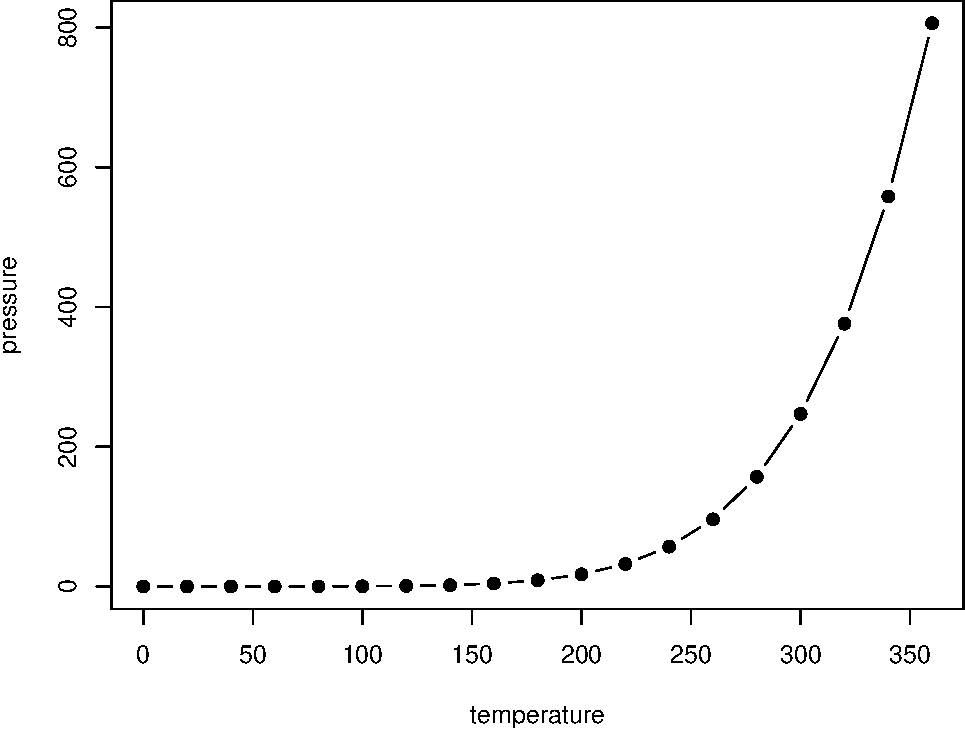
\includegraphics[width=0.8\linewidth]{bookdown-demo_files/figure-latex/nice-fig-1} 

}

\caption{Here is a nice figure!}\label{fig:nice-fig}
\end{figure}

Reference a figure by its code chunk label with the \texttt{fig:}
prefix, e.g., see Figure \ref{fig:nice-fig}. Similarly, you can
reference tables generated from \texttt{knitr::kable()}, e.g., see Table
\ref{tab:nice-tab}.

\begin{Shaded}
\begin{Highlighting}[]
\NormalTok{knitr::}\KeywordTok{kable}\NormalTok{(}
  \KeywordTok{head}\NormalTok{(iris, }\DecValTok{20}\NormalTok{), }\DataTypeTok{caption =} \StringTok{'Here is a nice table!'}\NormalTok{,}
  \DataTypeTok{booktabs =} \OtherTok{TRUE}
\NormalTok{)}
\end{Highlighting}
\end{Shaded}

\begin{table}

\caption{\label{tab:nice-tab}Here is a nice table!}
\centering
\begin{tabular}[t]{rrrrl}
\toprule
Sepal.Length & Sepal.Width & Petal.Length & Petal.Width & Species\\
\midrule
5.1 & 3.5 & 1.4 & 0.2 & setosa\\
4.9 & 3.0 & 1.4 & 0.2 & setosa\\
4.7 & 3.2 & 1.3 & 0.2 & setosa\\
4.6 & 3.1 & 1.5 & 0.2 & setosa\\
5.0 & 3.6 & 1.4 & 0.2 & setosa\\
\addlinespace
5.4 & 3.9 & 1.7 & 0.4 & setosa\\
4.6 & 3.4 & 1.4 & 0.3 & setosa\\
5.0 & 3.4 & 1.5 & 0.2 & setosa\\
4.4 & 2.9 & 1.4 & 0.2 & setosa\\
4.9 & 3.1 & 1.5 & 0.1 & setosa\\
\addlinespace
5.4 & 3.7 & 1.5 & 0.2 & setosa\\
4.8 & 3.4 & 1.6 & 0.2 & setosa\\
4.8 & 3.0 & 1.4 & 0.1 & setosa\\
4.3 & 3.0 & 1.1 & 0.1 & setosa\\
5.8 & 4.0 & 1.2 & 0.2 & setosa\\
\addlinespace
5.7 & 4.4 & 1.5 & 0.4 & setosa\\
5.4 & 3.9 & 1.3 & 0.4 & setosa\\
5.1 & 3.5 & 1.4 & 0.3 & setosa\\
5.7 & 3.8 & 1.7 & 0.3 & setosa\\
5.1 & 3.8 & 1.5 & 0.3 & setosa\\
\bottomrule
\end{tabular}
\end{table}

You can write citations, too. For example, we are using the
\textbf{bookdown} package \citep{R-bookdown} in this sample book, which
was built on top of R Markdown and \textbf{knitr} \citep{xie2015}.

\chapter{Installation}\label{install}

\texttt{saemix} can be installed and used on several platforms.
Installation can range from easy to challenging, depending on the
platform. We are in the process of streamlining this process, and any
help or suggestions are greatly appreciated!

\section{\texorpdfstring{\texttt{saemix}}{saemix}}\label{saemix}

Information on how to install `saemix' and its dependencies on different
platforms can be found on the
\href{https://saemixdevelopment.github.io/saemix/index.html}{\texttt{saemix}
pkgdown site}. Separate information can be found on
\href{https://saemixdevelopment.github.io/RxODE/index.html}{\texttt{RxODE}
pkgdown site}.

\subsection{Installation via GitHub}\label{installation-via-github}

To Complete

\section{\texorpdfstring{\texttt{shinyMixR}: project management
tool}{shinyMixR: project management tool}}\label{shinymixr-project-management-tool}

A user-friendly tool was developed for \texttt{saemix} based on
\href{http://shiny.rstudio.com/}{\texttt{Shiny}}

\chapter{User guide}\label{userguide}

\section{Posters, Presentations and
Publications}\label{posters-presentations-and-publications}

\begin{itemize}
\tightlist
\item
  PAGE 2016, City, Country: TestSlides
\end{itemize}

Various other publications can be found
\href{https://github.com/saemixdevelopment/Publications}{here}.

\chapter{Case Studies}\label{casestudies}

Some basic Case Studies are demonstrated in this chapter; the vignettes
will be discussing the application in more depth.

\section{\texorpdfstring{\texttt{saemix}}{saemix}}\label{saemix-1}

\begin{Shaded}
\begin{Highlighting}[]
\KeywordTok{library}\NormalTok{(saemix)}
\NormalTok{?saemix}
\end{Highlighting}
\end{Shaded}

\subsection{Rationale}\label{rationale}

\texttt{saemix} estimation routines have their own way of specifying
models.

\textbf{Initial Values}

\texttt{saemix} models are contained in a R function with two blocks:

\begin{Shaded}
\begin{Highlighting}[]
\NormalTok{Some R Code}
\end{Highlighting}
\end{Shaded}

\subsection{Some examples}\label{some-examples}

\subsubsection{A two-compartment PK
model}\label{a-two-compartment-pk-model}

The model:

\begin{Shaded}
\begin{Highlighting}[]
\NormalTok{theomodel <-}\StringTok{ }\NormalTok{function() \{}
  \KeywordTok{ini}\NormalTok{(\{}
    \NormalTok{tka <-}\StringTok{ }\KeywordTok{log}\NormalTok{(}\FloatTok{1.14}\NormalTok{)}
    \NormalTok{tcl <-}\StringTok{ }\KeywordTok{log}\NormalTok{(}\FloatTok{0.0190}\NormalTok{)}
    \NormalTok{tv2  <-}\StringTok{ }\KeywordTok{log}\NormalTok{(}\FloatTok{2.12}\NormalTok{)}
    \NormalTok{tv3  <-}\StringTok{ }\KeywordTok{log}\NormalTok{(}\FloatTok{20.4}\NormalTok{)}
    \NormalTok{tq   <-}\StringTok{ }\KeywordTok{log}\NormalTok{(}\FloatTok{0.383}\NormalTok{)}
    \NormalTok{wteff  <-}\StringTok{ }\FloatTok{0.35}
    \NormalTok{sexeff <-}\StringTok{ }\NormalTok{-}\FloatTok{0.2}
    \NormalTok{eta.ka ~}\StringTok{ }\DecValTok{1}
    \NormalTok{eta.cl ~}\StringTok{ }\DecValTok{1}
    \NormalTok{eta.v2 ~}\StringTok{ }\DecValTok{1}
    \NormalTok{eta.v3 ~}\StringTok{ }\DecValTok{1}
    \NormalTok{eta.q ~}\StringTok{ }\DecValTok{1}
    \NormalTok{prop.err <-}\StringTok{ }\FloatTok{0.075}
  \NormalTok{\})}
  \KeywordTok{model}\NormalTok{(\{}
    \NormalTok{ka <-}\StringTok{ }\KeywordTok{exp}\NormalTok{(tka +}\StringTok{ }\NormalTok{eta.ka)}
    \NormalTok{cl <-}\StringTok{ }\KeywordTok{exp}\NormalTok{(tcl +}\StringTok{ }\NormalTok{wteff*lWT +}\StringTok{ }\NormalTok{eta.cl)}
    \NormalTok{v2 <-}\StringTok{ }\KeywordTok{exp}\NormalTok{(tv2 +}\StringTok{ }\NormalTok{sexeff*SEX +}\StringTok{ }\NormalTok{eta.v2)}
    \NormalTok{v3 <-}\StringTok{ }\KeywordTok{exp}\NormalTok{(tv3 +}\StringTok{ }\NormalTok{eta.v3)}
    \NormalTok{q  <-}\StringTok{ }\KeywordTok{exp}\NormalTok{(tq +}\StringTok{ }\NormalTok{eta.q)}
    \NormalTok{d/}\KeywordTok{dt}\NormalTok{(depot) =}\StringTok{ }\NormalTok{-ka *}\StringTok{ }\NormalTok{depot}
    \NormalTok{d/}\KeywordTok{dt}\NormalTok{(center) =}\StringTok{ }\NormalTok{ka *}\StringTok{ }\NormalTok{depot -}\StringTok{ }\NormalTok{cl /}\StringTok{ }\NormalTok{v2 *}\StringTok{ }\NormalTok{center +}\StringTok{ }\NormalTok{q/v3 *}\StringTok{ }\NormalTok{periph -}\StringTok{ }\NormalTok{q/v2 *}\StringTok{ }\NormalTok{center}
    \NormalTok{d/}\KeywordTok{dt}\NormalTok{(periph) =}\StringTok{ }\NormalTok{q/v2 *}\StringTok{ }\NormalTok{center -}\StringTok{ }\NormalTok{q/v3 *}\StringTok{ }\NormalTok{periph}
    \NormalTok{cp =}\StringTok{ }\NormalTok{center /}\StringTok{ }\NormalTok{v2}
    \NormalTok{cp ~}\StringTok{ }\KeywordTok{prop}\NormalTok{(prop.err)}
  \NormalTok{\})}
\NormalTok{\}}

\NormalTok{fit <-}\StringTok{ }\KeywordTok{saemix}\NormalTok{()}
\end{Highlighting}
\end{Shaded}

\chapter*{Contacts}\label{contacts}
\addcontentsline{toc}{chapter}{Contacts}

You can label chapter and section titles using \texttt{\{\#label\}}
after them, e.g., we can reference Chapter \ref{intro}. If you do not
manually label them, there will be automatic labels anyway, e.g.,
Chapter \ref{methods}.

Figures and tables with captions will be placed in \texttt{figure} and
\texttt{table} environments, respectively.

\bibliography{book.bib,packages.bib}

\end{document}
